\section{Software}
To measure an object with a camera, the software has to perform lots of different tasks in a certain period of time.
First off, it needs to take the non-linear distortions of the camera into account.
After that, some sort of trigger is needed, to check the frames for objects and pass a frame on, if an object is within the frame.
Now, the software needs to detect a known pattern on the plane where the object lies.
With the known distances of the pattern, a pixel per metric unit can be calculated.
This unit describes, how many pixels (depended on the camera-pattern distance) fit into one metric unit (in this case mm) and is used to convert dimensions in pixel to dimensions in mm and vice versa.
This pattern can also be used to calculate a transformation matrix which compensates slight angular errors resulting from an imprecise mounting of the camera.
After all these steps, the object has to be recognized and
finally, the dimensions of the object have to be estimated.

All these steps are described in more detail in the following sections.
It is important to keep in mind, that OpenCV uses a coordinate-system with a switched $x-$ and $y-$axis. 

% listing to python code
\definecolor{codegray}{rgb}{0.5,0.5,0.5}
\definecolor{backcolour}{rgb}{0.95,0.95,0.92}

\lstdefinestyle{mystyle}{
	language=Python,
	backgroundcolor=\color{backcolour},   
	commentstyle=\color{purple},
	keywordstyle=\color{blue!50!black},
	numberstyle=\tiny\color{white},
	stringstyle=\color{green!50!black},
	basicstyle=\footnotesize\ttfamily,
	breakatwhitespace=false,         
	breaklines=true,                 
	captionpos=b,                    
	keepspaces=true,                 
	numbers=left,                    
	numbersep=2pt,                  
	showspaces=false,                
	showstringspaces=false,
	showtabs=false,                  
	tabsize=2,
	emph={int, char, double, float, range, len, bytes},
	emphstyle=\color{violet},
	morekeywords={as}
}
\lstset{style=mystyle}

\subsection{Initialization}
In the first step, global variables like frame height \texttt{h} and width \texttt{w} are defined.
The camera intrinsics, which where obtained in the calibration previously are loaded from a .txt-file into the script, which are used to compute the \texttt{map\_x} and \text{map\_y}.
This is shown in the following code snipped.
\begin{lstlisting}
	# load calibration parameters
	mtx = np.loadtxt('mtx_normal.txt')
	dst = np.loadtxt('dist_normal.txt')

	# get calibration map
	map_x, map_y = cv2.initUndistortRectifyMap(mtx, dst, None, mtx,
	                                           (w, h), cv2.CV_32FC1)
\end{lstlisting}
These are two maps are arrays which contain the inversion of the distortion for each image point.
This calculation has to be done only one time before entering the main loop and can be used efficiently afterwards to undistort points in the image.

There are two more variables the user can define, depended on the environment, geometry pattern and camera-glass plate distance.
The variable \texttt{sep} splits the frame horizontally into three stripes and the variable \texttt{vec} does the same thing vertically.
Both \texttt{sep} and \texttt{vec} are used later in the code, to define sections in which the either the geometry pattern or the object to measure is searched.
Figure \ref{development:sep} visualizes these two variables.
\begin{figure}[ht]
	\centering
	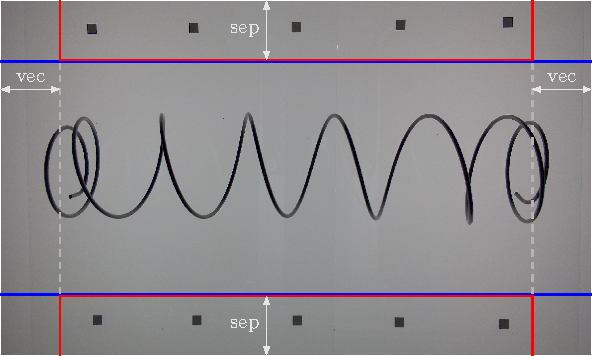
\includegraphics[width=0.9\textwidth]{3-development/software/images/sep.pdf}
	\caption{Different image sections.\label{development:sep}}
\end{figure}
The red section is the part of the image, in which the geometry pattern is searched and the blue stripe in the middle defines the section where the object has to be.

\subsection{Trigger}
The trigger is implemented as a function which reads frames continuously and computes the variance of the first column.
If this variance is low, the whole column is uniform and therefore no spring is entering the frame (the springs are moving from left to right).
If the variance is higher than a certain threshold, it is assumed that an object is entering the frame and the trigger searches in the next 5 frames for an image in which contains the whole object.
This is done again by calculating the variances of three more columns, two around the center and the last column of the image.
If a frame contains the whole object, it is returned to the main loop to make further calculations.
This way it is possible to run the trigger at a max of 22\,fps.

Turns out that this is not fast enough.
While testing the software, in about half of the cases the problem occurred, that the object could be detected entering the frame, but moved to fast and was therefore the next frame already in partly outside.
In such a case, no image contains the whole object and no measurements can be done.

\subsection{Threshold and edge detection}
To measure a object passing the camera's field of view, the outlines of the object are needed.
The challenge here is to find the edges of an object with little computing power in a time-span such that the measurement time does not become useless.
For further processing the edges have to be represented by an one pixel thick line.
This section shows the used method and implementation of the used edge detection.
The \acs{ISP}driver of the Jetson Nano is used in the automatic mode.
In this configuration the \acs{isp} tries to keep the mean of the image close to the value 127, which resembles the middle of its range. Since the communication with the camera driver over Python is somewhat complicated, the camera is only used in automatic mode.

\subsubsection{Threshold}
To determine a good threshold method, a short look at the histogram is the first step to success.
With the backlight, it can be expected to have a clear difference between foreground and background of the image.
Two images with it's histogram are shown in Figure \ref{development::thre}.
\begin{figure}[ht]
	\centering
	\subfigure[\label{development:thre1}]{\fbox{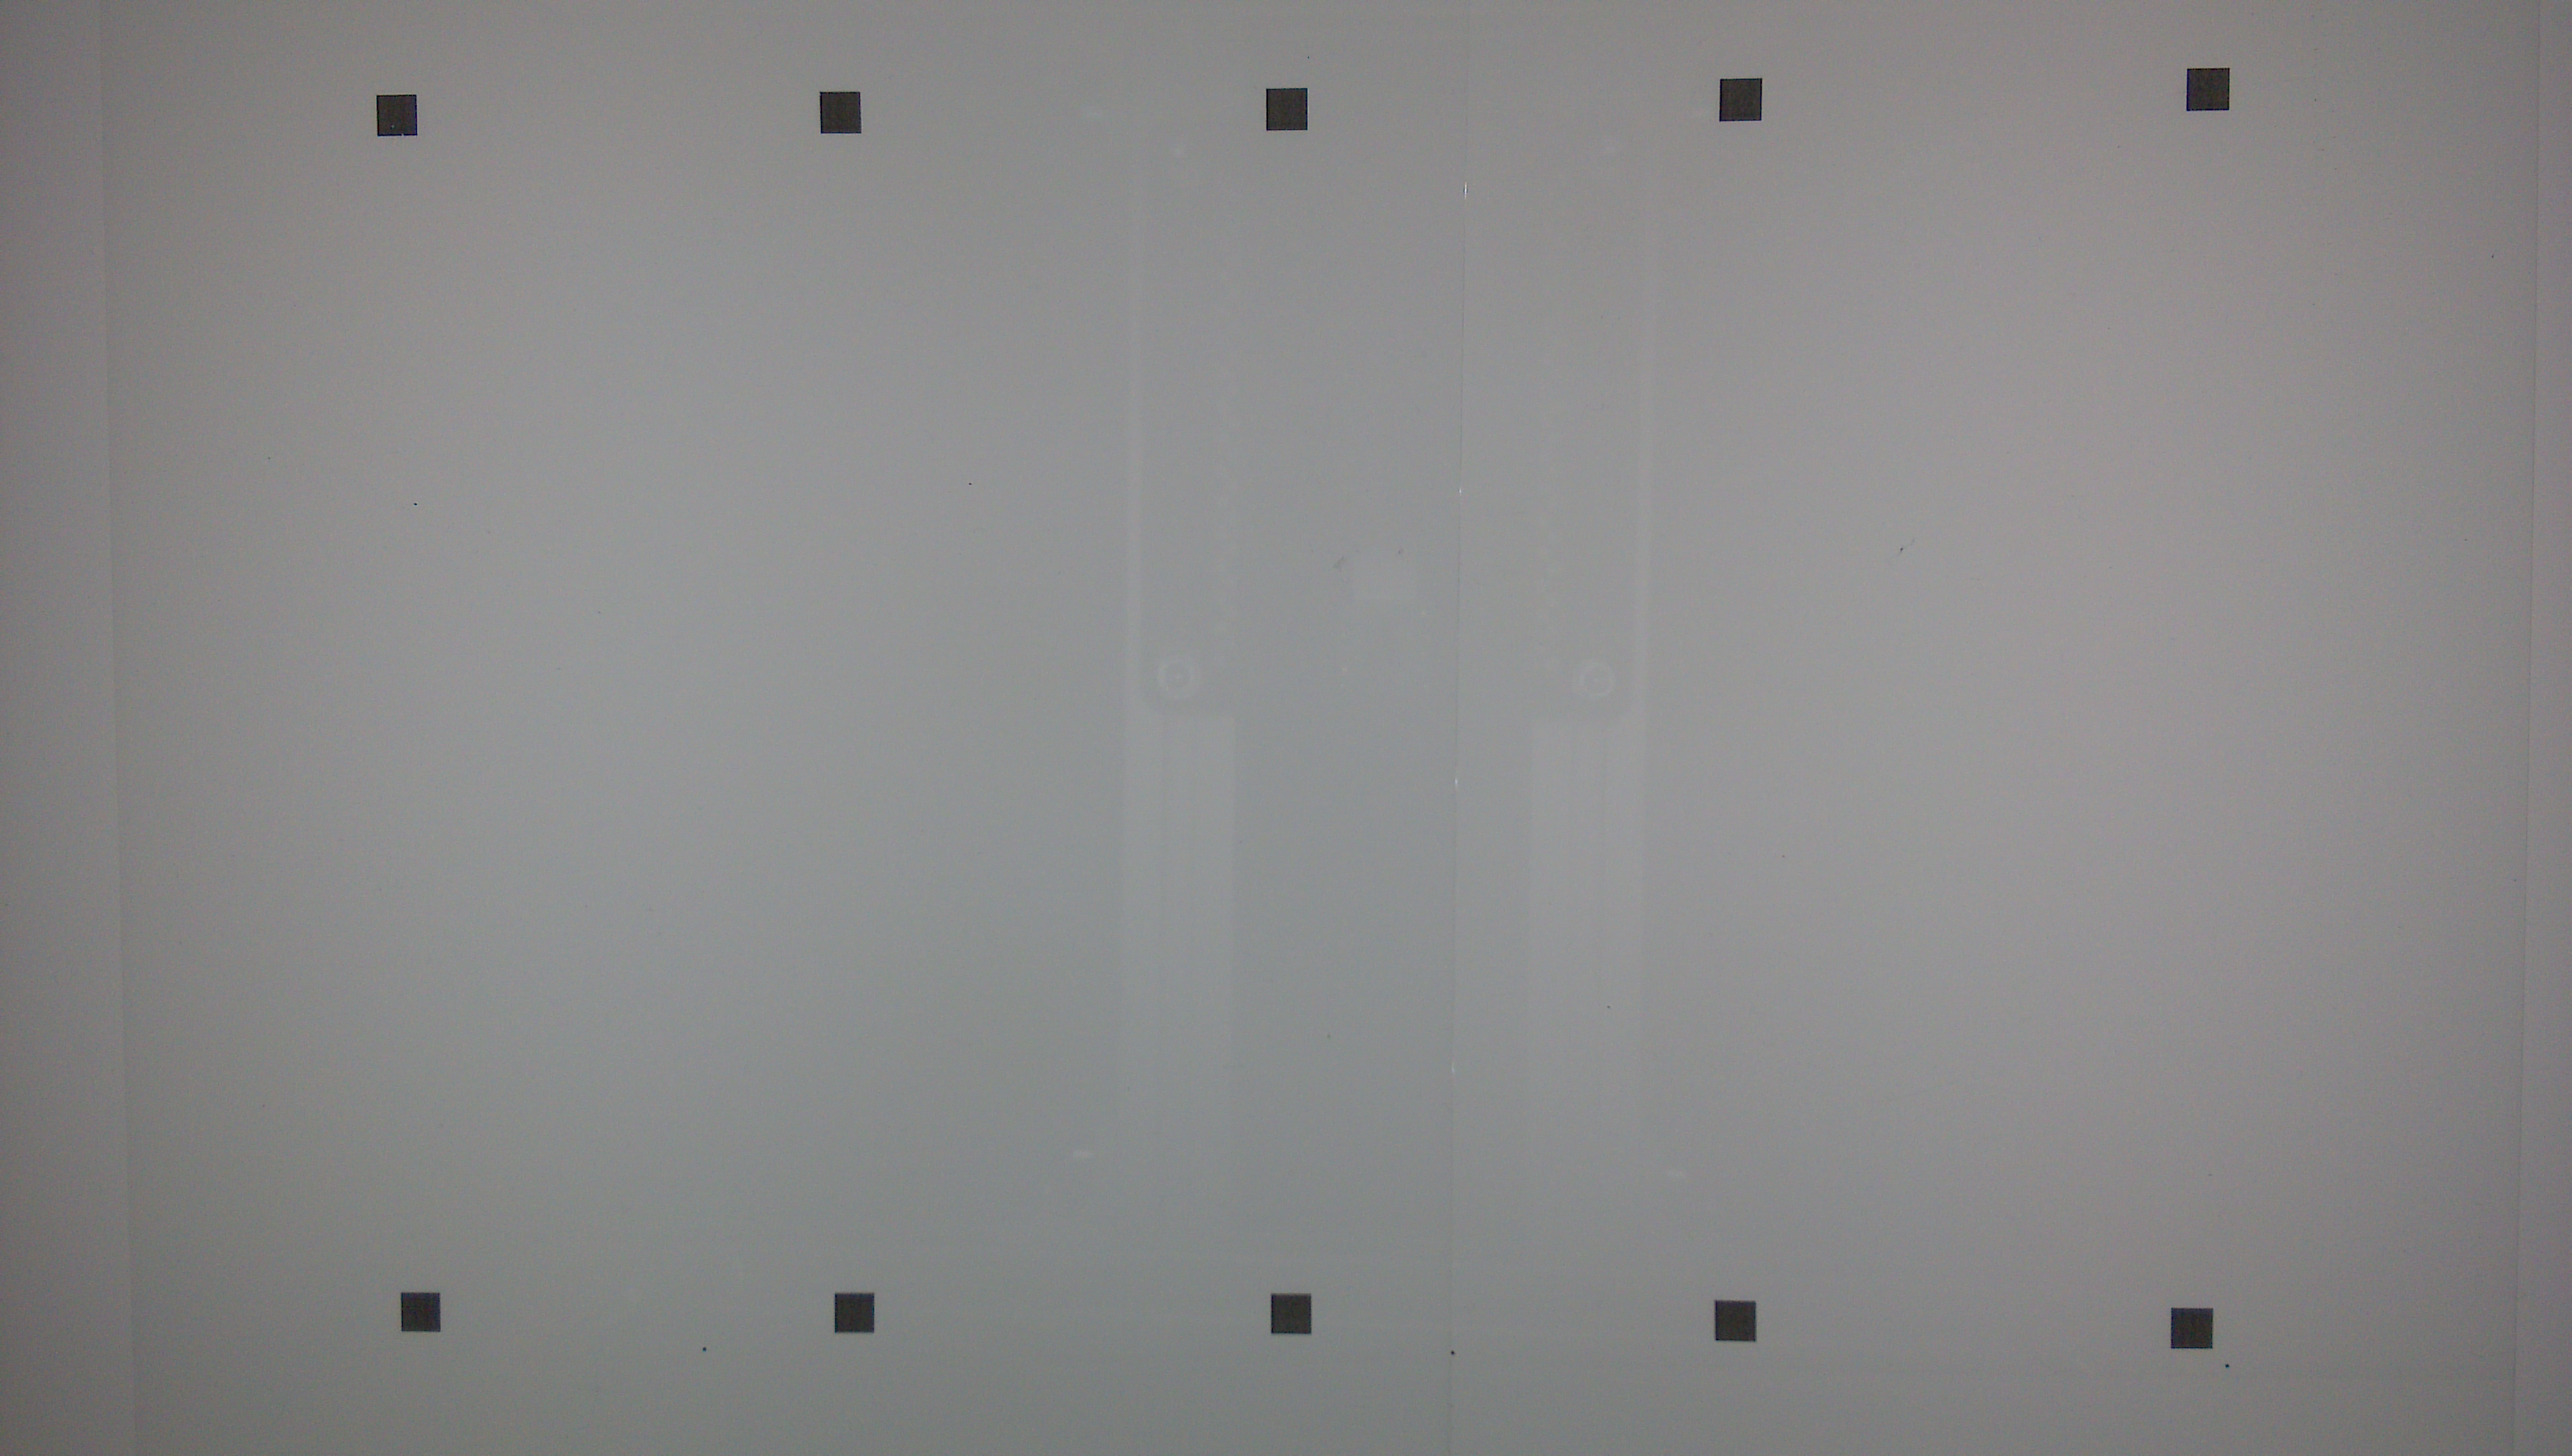
\includegraphics[width=0.45\linewidth, height=5cm]{3-development/threshold/im0.png}}}
	\subfigure[\label{development:thre2}]{\fbox{\includegraphics[width=0.45\linewidth, height=5cm]{3-development/threshold/hist_pattern2.pdf}}}
	\subfigure[\label{development:thre3}]{\fbox{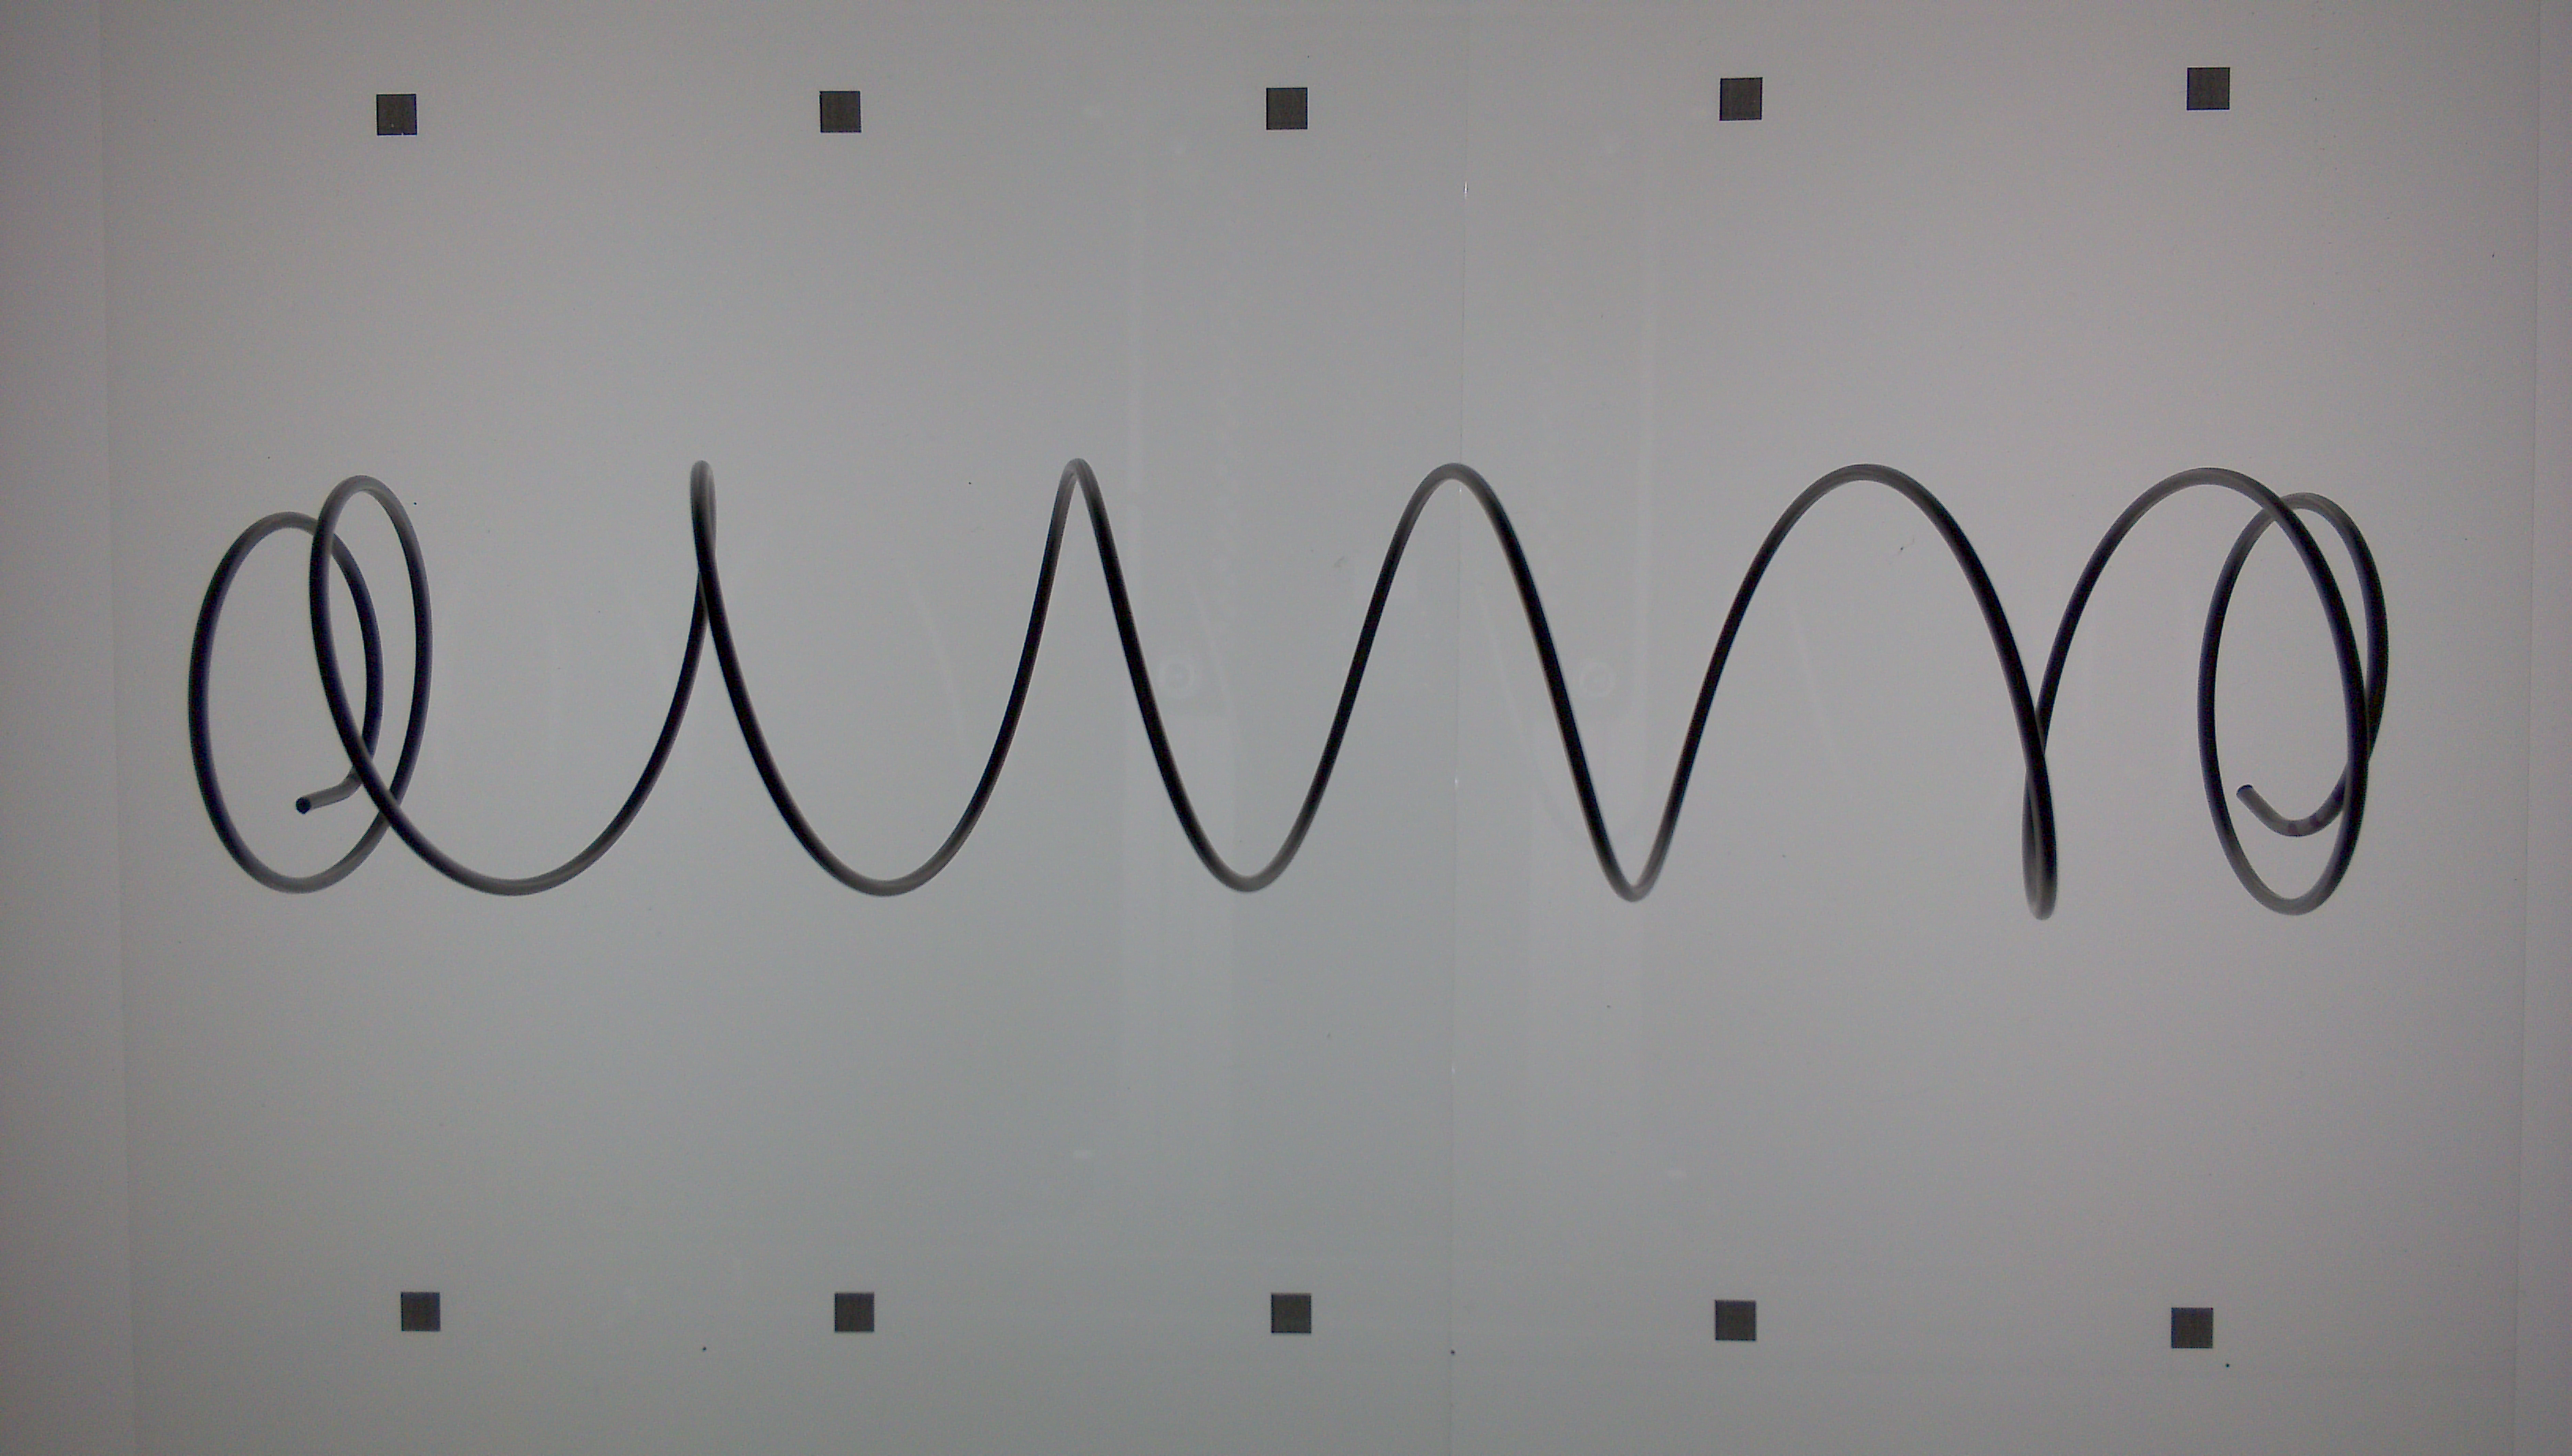
\includegraphics[width=0.45\linewidth, height=5cm]{3-development/threshold/im1.png}}}
	\subfigure[\label{development:thre4}]{\fbox{\includegraphics[width=0.45\linewidth, height=5cm]{3-development/threshold/hist_feder2.pdf}}}
	\caption{Histogram of the reference pattern and a spring in frame.\label{development:thre}}	
\end{figure}
In Subfigure \ref{development:thre1}, the backlight is running and the calibration pattern is in place but there is no object to measure.
The corresponding histogram \ref{development:thre2} shows that nearly every pixel belongs to the background (white) which is between the intensity 100 and 155.
If an object enters the frame, it is displayed as black and we get more small values.
This shift is also reproduced by the variance.
The mean itself is getting corrected by the \acs{isp} and can not be used to detect if an object is in the image or not.

The obvious answer for a threshold would now be to just cut the image around the value 100.
But with the automatic \acs{ISP}, there is a good chance to loose important information if there is no adaptive threshold.
Since the goal is to get as much information as possible from the edges, this little bit of noise should be be handled.
The method which produced the best results with a backlight was the triangle method \ref{theory:triangle}.

The triangle method calculates the value 112 on the given image in Subfigure \ref{development:thre3} which, using a binary threshold, results in the binary image in Figure \ref{development:thresh}.
It is visible that we get a lot of noise in the edges of the resulting picture.
\begin{center}
	\centering
	\fbox{\includegraphics[width=0.9\linewidth]{3-development/threshold/threshold.png}}
	\captionof{figure}{Image after triangle threshold with value 112.}
	\label{development:thresh}
\end{center}
Since the noise occurs only in the edges of the image, it can dealt with ease.
The focus lies more on the pattern and spring which should lose as few information as possible.

Another very popular method for an global adaptive threshold is the otsu algorithm. Otsu's goal is to maximize the variance of the fore- and background in a image as good as possible in the histogram. Also known as the between-class variance. The result of an otsu threshold on the given image \ref{development:thre3} can be seen in the image in Figure \ref{development:otsu}. On the first sight it looks pretty clean and no noise is visible. Which leads to think that the otsu should be a good algorithm for this problem. But if the images in Figures \ref{development:triangle} and \ref{development:otsu} are investigated a little bit closer and compared directly it shows some disadvantage of the otsu which can not be corrected afterwards.
\begin{figure}[ht]
	\centering
	\subfigure[\label{development:triangle}]{\fbox{\includegraphics[width=0.44\linewidth, height=5cm]{3-development/threshold/threshold.png}}}
	\subfigure[\label{development:otsu}]{\fbox{\includegraphics[width=0.44\linewidth, height=5cm]{3-development/threshold/otsu.png}}}
	\subfigure[\label{development:difference}]{\fbox{\includegraphics[width=0.9\linewidth]{3-development/threshold/diff.png}}}
	\caption{Comparison between otsu and triangle threshold.\label{development:diff}}	
\end{figure}
If we look closely at the silhouette of the spring after the otsu threshold it seems that in some parts of the spring are disappearing. While the image which is thresholded with the triangle method it seems that far less information is lost. To better illustrate this effect the otsu image is subtracted by the triangle one which results in the difference image \ref{development:difference}.  
Now the difference clearly shows how much information is lost on the edges of the spring and even on the pattern. This information once lost can not be obtained again. With this in mind the otsu seems unsuitable for this problem.
The source of the problem itself is that the spring reflects the stray light of the backlight. The stray light is produced by two effects, one is the diffusion film which is only 4\,mm away from the spring. The second one is the reflected light from the construction itself. Meaning the top of the construction where the camera is mounted reflects some amount back on the spring. These two sources of stray light are leading to the spring being illuminated enough from the top, that some brightness values captured by the camera sensor are the same in the edges of the image as parts of spring.
Hardware improvements to minimize this problem would be to use light control filters which results in higher hardware cost. Another way would be to increase the distance between the glass plate and the diffusion filter.
In addition to these two solutions, the backlight could be changed in order to reduce the vignetting of the camera.
Vignetting could also be handled in software.
Since the background of the image stays the same, it is possible to subtract the background of the image first eliminating the noise in the corner. The down side in correcting the brightness in a complex manner is the time spent doing it.
Since every pixel has to be corrected, it takes a good amount of time for the whole image.
This would reduce the speed of the whole measurement drastically.

\subsubsection{Edge detection}   
To obtain the edge from a thresholded image, morphological algorithms are should be used since they are very fast. Thanks to the good threshold results which also uses quite some time to calculate it, is now fairly easy to get the edge of the spring. To extract the boundary of the spring we use a $3\times 3$ kernel to erode the given image. The kernel $K$ is shaped as followed:
\begin{center}
	\setlength{\tabcolsep}{0.5em} % for the horizontal padding
	{\renewcommand{\arraystretch}{1.2}
		\begin{tabular}{|c|c|c|}
			\hline
			1&1&1\\
			\hline
			1&1&1\\
			\hline
			1&1&1\\
			\hline
		\end{tabular}
	}
\end{center}

This kernel $K$ is used to erode the image and subtract the eroded image from the starting image. Lets name the thresholded image $T$. The math done is 
\begin{align*}
E = T-(T\ominus K)
\end{align*}
returning the image containing all the edges $E$. In our example picture, the resulting picture $E$ is displayed in the image \ref{development:edge}.\\
\begin{figure}[ht]
	\centering
	\fbox{\includegraphics[width=0.9\linewidth]{3-development/threshold/edge.png}}
	\caption{Edges of given image with morphological detection}
	\label{development:edge}
\end{figure}
As we can see from the image in Figure\ref{development:edge}, noise which leads to bigger pixel areas than the 3x3 kernel can also be seen as edges. But since we know that our spring can't be located outside of our separation (definde with \texttt{sep}), the corners can just be ignored.
This shows the following code snipped.
\begin{lstlisting}
	ret3, thresh = cv2.threshold(img, 0, 255, cv2.THRESH_BINARY +
	                             cv2.THRESH_TRIANGLE)
	erode = cv2.erode(thresh, kernel, iterations=1)
	return cv2.subtract(thresh, erode)
\end{lstlisting} 
Note that this code only gives the wanted result if the image is converted into a grayscale image with the OpenCV function \texttt{cv.cvtColor(img, cv2.COLOR\_BGR2GRAY)}.
If the image is loaded with the OpenCV function \texttt{cv.imread(file,0)} the frame is imported directly as a grayscale image. For unknown reasons this two functions are converting the image differently, resulting in different results.

\subsection{Pattern recognition}
The binary image containing the edges is now used to search for the contours of the geometry pattern on the plane.
The pattern consists of 10 rectangles printed on a transparent sheet.
First, it is necessary to find all the contours \texttt{with cv2.findCountours()} inside the two boundaries defined by \texttt{vec} and \texttt{sep}.
This function returns an array of arrays, in which coordinates of the pixels, belonging to one contour are stored.

Because the edge detection is not perfect, some contours will be found which do not belong to the pattern.
By using the area of each contour as basis of decision making, it is possible to remove invalid contours.
This is done in with in the following code segment, where \texttt{cnts\_upper} and \texttt{cnts\_lower} are array storing the contours.
\begin{lstlisting}
	# only keep valid contours
	cnts_upper = remove_contours(cnts_upper, 2600, 3400)
	cnts_lower = remove_contours(cnts_lower, 2600, 3400)
\end{lstlisting}
If an area of a contour is not between $2600$ and $3400\,$ pixels, the contour is removed.
These two values are of course depended on the rectangle size used and the distance from the camera to the plane.

These left contours (basically an array of points) can be undistorted using \texttt{map\_x} and \texttt{map\_y}.

Now a rectangle is fitted over each contour (with \texttt{cv2.minAreaRect()}).
The center of each rectangle is stored in an array.
These points are here called image-points (in the code as variable \texttt{imgp}).

It is now possible to calculate the pixel per metric unit (\texttt{ppm}) by computing a distance between two image points in pixels and then dividing this distance by the real pattern distance in mm.
In fact it is even more reasonable to do this for a lot of distances and taking the mean of each \texttt{ppm}, assuming that errors in the pattern detection will cancel each other out.

After that, a numpy-array which describes the same pattern how it should appear on the plane if the camera was mounted correctly is generated
This points are here called object-points (\texttt{objp}).
In python this looks like the following code snipped.
\begin{lstlisting}
	objp = np.array([[-110 * ppm + cx, -75 * ppm + cy],
	                 [ -55 * ppm + cx, -75 * ppm + cy],
	                 [             cx, -75 * ppm + cy],
	                 [  55 * ppm + cx, -75 * ppm + cy],
	                 [ 110 * ppm + cx, -75 * ppm + cy],
	                 [-110 * ppm + cx,  75 * ppm + cy],
	                 [ -55 * ppm + cx,  75 * ppm + cy],
	                 [             cx,  75 * ppm + cy],
	                 [  55 * ppm + cx,  75 * ppm + cy],
	                 [ 110 * ppm + cx,  75 * ppm + cy]], dtype=np.float32)
\end{lstlisting}
The variables \texttt{cx} and \texttt{cy} are the coordinates of the calibrated principal point of the camera.
The datatype of the entries is forced to float32 because some OpenCV functions later used do not accept other types.

Now that we have our image- and object points, a perspective transformation matrix can be calculated which looks like the following code.
\begin{lstlisting}
	 T, _ = cv2.findHomography(imgp, objp, method=0)
\end{lstlisting}
This function calculates \texttt{T} in such a way, that the image-points are mapped to the object points using the least-square method (set by \texttt{method=0}).
Or more mathematical:
\begin{align*}
	\begin{pmatrix}
	x_{\text{obj}, i}\\
	y_{\text{obj}, i}\\
	1
	\end{pmatrix}\sim T
	\begin{pmatrix}
	x_{\text{img}, i}\\
	y_{\text{img}, i}\\
	1
	\end{pmatrix}	
\end{align*}
such that
\begin{align*}
	\sum_{i}\left(x_{\text{obj},i}-\frac{T_{11}x_{\text{img},i}+T_{12}y_{\text{img},i}+T_{13}}{T_{31}x_{\text{img},i}+T_{32}y_{\text{img},i}+T_{33}}\right)^2+
	\sum_{i}\left(y_{\text{obj},i}-\frac{T_{21}x_{\text{img},i}+T_{22}y_{\text{img},i}+T_{23}}{T_{31}x_{\text{img},i}+T_{32}y_{\text{img},i}+T_{33}}\right)^2
\end{align*}
is minimized \cite{cv_calib}.
The matrix \texttt{T} is later used to compensate the error made because of the camera mounting. 

\subsection{Object recognition and geometry estimation}
Now that these first calculations are made, the object is detected just like the pattern.
With the function \texttt{cv2.findcontours()} all contours are extracted from the image with the edges, but this time in between the separation \texttt{sep}.
And again like before, invalid contours are removed, based on their area and undistorted.
Because the object in this case is a steel spring, the contours are somewhat complicated and it is possible, that contours are found, which are not connected to each other but definitely belong to the spring.
In this case, the OpenCV function returns them as different contours and it is therefore necessary to combine all returned contours into one single array.
The following code shows how this is achieved in addition with applying the rectification transform and fitting a rectangle over it.
\begin{lstlisting}
	# combine contours to one
	cnts_m = np.concatenate(cnts_m, axis=0).astype(np.float64)
	
	# warp perspective of the contours
	cnts_m = cv2.perspectiveTransform(cnts_m, T)
	
	# minimum area rectangle around cnts_m
	box = cv2.minAreaRect(cnts_m.astype(np.float32))
\end{lstlisting}
\texttt{cnts\_m} are here the contours found previously.
Since now a rectangle with its coordinates is know, everything is ready for the actual geometry estimation.

Because no telecentric objective is used, one has to consider, that the camera looks at the edges of the object in a slight angle.
For simplicity, it is at this point assumed that the steel spring as a cylinder, which is aligned horizontal in the image plane.
A cut through the center of this cylinder along the $y$-axis (OpenCV coordinates) is show in figure \ref{development:diameter}.
\begin{figure}[ht]
	\centering
	\includegraphics[width=0.9\linewidth]{3-development/software/images/diameter_estimation.pdf}
	\caption{Steel spring cut through the center along $y$-axis.\label{development:diameter}}
\end{figure}
$x_{\text{obj}}$ denotes the center of the object (spring) while $cx$ is the $x-$coordinate of the calibrated principal point.
The distance from the camera to the plane can be calculated by using the theorem of intersecting lines, since the focal length and pixel-size are known from the data-sheet of the camera and the pixel per metric unit has been calculated previously.
Also known are the two observed points on the plane $(x_{\text{obj}}, y_p^{(1)})$ and $(x_{\text{obj}}, y_p^{(2)})$.

The distances from these two points on the plane to the camera and to each other can now be calculated as
\begin{align*}
	d_{1}&=\sqrt{(c_y-y_p^{(1)})^2+h^2}\\
	d_{2}&=\sqrt{(c_y-y_p^{(2)})^2+h^2}\\
	d_{3}&=y_p^{(2)}-y_p^{(1)}.
\end{align*}
The distance must of course have the same units, in this case all distances in pixel where first converted to distances in mm.

This provides enough information to apply the geometry of in-circles \cite{incircles} to calculate the radius of the object as
\begin{align*}
	r=\sqrt{\frac{(s-d_1)(s-d_2)(s-d_3)}{s}}
\end{align*}
with
\begin{align*}
	s=\frac{d_1+d_2+d_3}{2}.
\end{align*}

A similar principle is applied to calculate the length of the object.
Figure \ref{development:length} where again
$y_{\text{obj}}$ denotes the center of the object (spring) while $c_x$ is the $x-$coordinate of the calibrated principal point.
\begin{figure}[ht]
	\centering
	\includegraphics[width=0.9\linewidth]{3-development/software/images/length_estimation.pdf}
	\caption{Steel spring cut through the center along $x$-axis.\label{development:length}}
\end{figure}
Observed are the two points on the plane $(x_p^{(1)}\quad y_{\text{obj}})$ and $(x_p^{(2)}\quad y_{\text{obj}})$.
But simply taking the difference of $x_p^{(1)}$ and $x_p^{(2)}$ result in to long length estimation.

Since $h$ is know, and $D$ has been calculated previously ($D=2r$), the theorem of intersecting lines allows one now to make the correction from the coordinates on the plane ($x_p^{(k)}$) to the points on the edge ($x_c^{(k)}$).

Mathematically expressed this results in
\begin{align*}
	\frac{c_x-x_c^{(k)}}{c_x-x_p^{(k)}}=\frac{h-D}{h}\quad\Leftrightarrow\quad
	x_c^{(k)}=\frac{h-D}{h}(c_x-x_p^{(k)}).
\end{align*}
After this correction the length can be calculated as
\begin{align*}
	L=x_c^{(2)}-x_c^{(1)}.
\end{align*}

These calculations are only accurate, if the object is placed horizontal in the frame.
In order to make accurate estimations even if the object is slightly rotated, the angle ($\theta$) between the minimum area rectangle found around the object and the horizontal has to be calculated.

The object or respectively the rectangle (the four corner points) has to be moved to the coordinate origin by removing the center and then rotated.
This transformation can be expressed as
\begin{align*}
	\begin{pmatrix}
	x'\\
	y'\\
	\end{pmatrix}=
	\begin{pmatrix}
	\cos(\theta)&-\sin(\theta)\\
	\sin(\theta)&\cos(\theta)
	\end{pmatrix}
	\begin{pmatrix}
	x-x_{\text{obj}}\\
	y-y_{\text{obj}}\\
	\end{pmatrix},	
\end{align*}
where $(x\quad y)^T$ are coordinates of the points of the object, $(x'\quad y')^T$ are transformed coordinates and $(x_{\text{obj}}, y_{\text{obj}})$ are again the coordinates of the center of the object, or respectively the min area rectangle.
By applying this transformation beforehand, the geometry estimation is independent of the the angle the object has to the horizontal. 

\subsection{Compensation of the rolling shutter}
The compensation of the rolling shutter is straight forward.
The Raspberry Pi Camera has a rolling shutter which stores the pixel values row per row (horizontal).
The effect this has in the image can be seen in Figure \ref{development:rolling}.
\begin{figure}[ht]
	\centering
	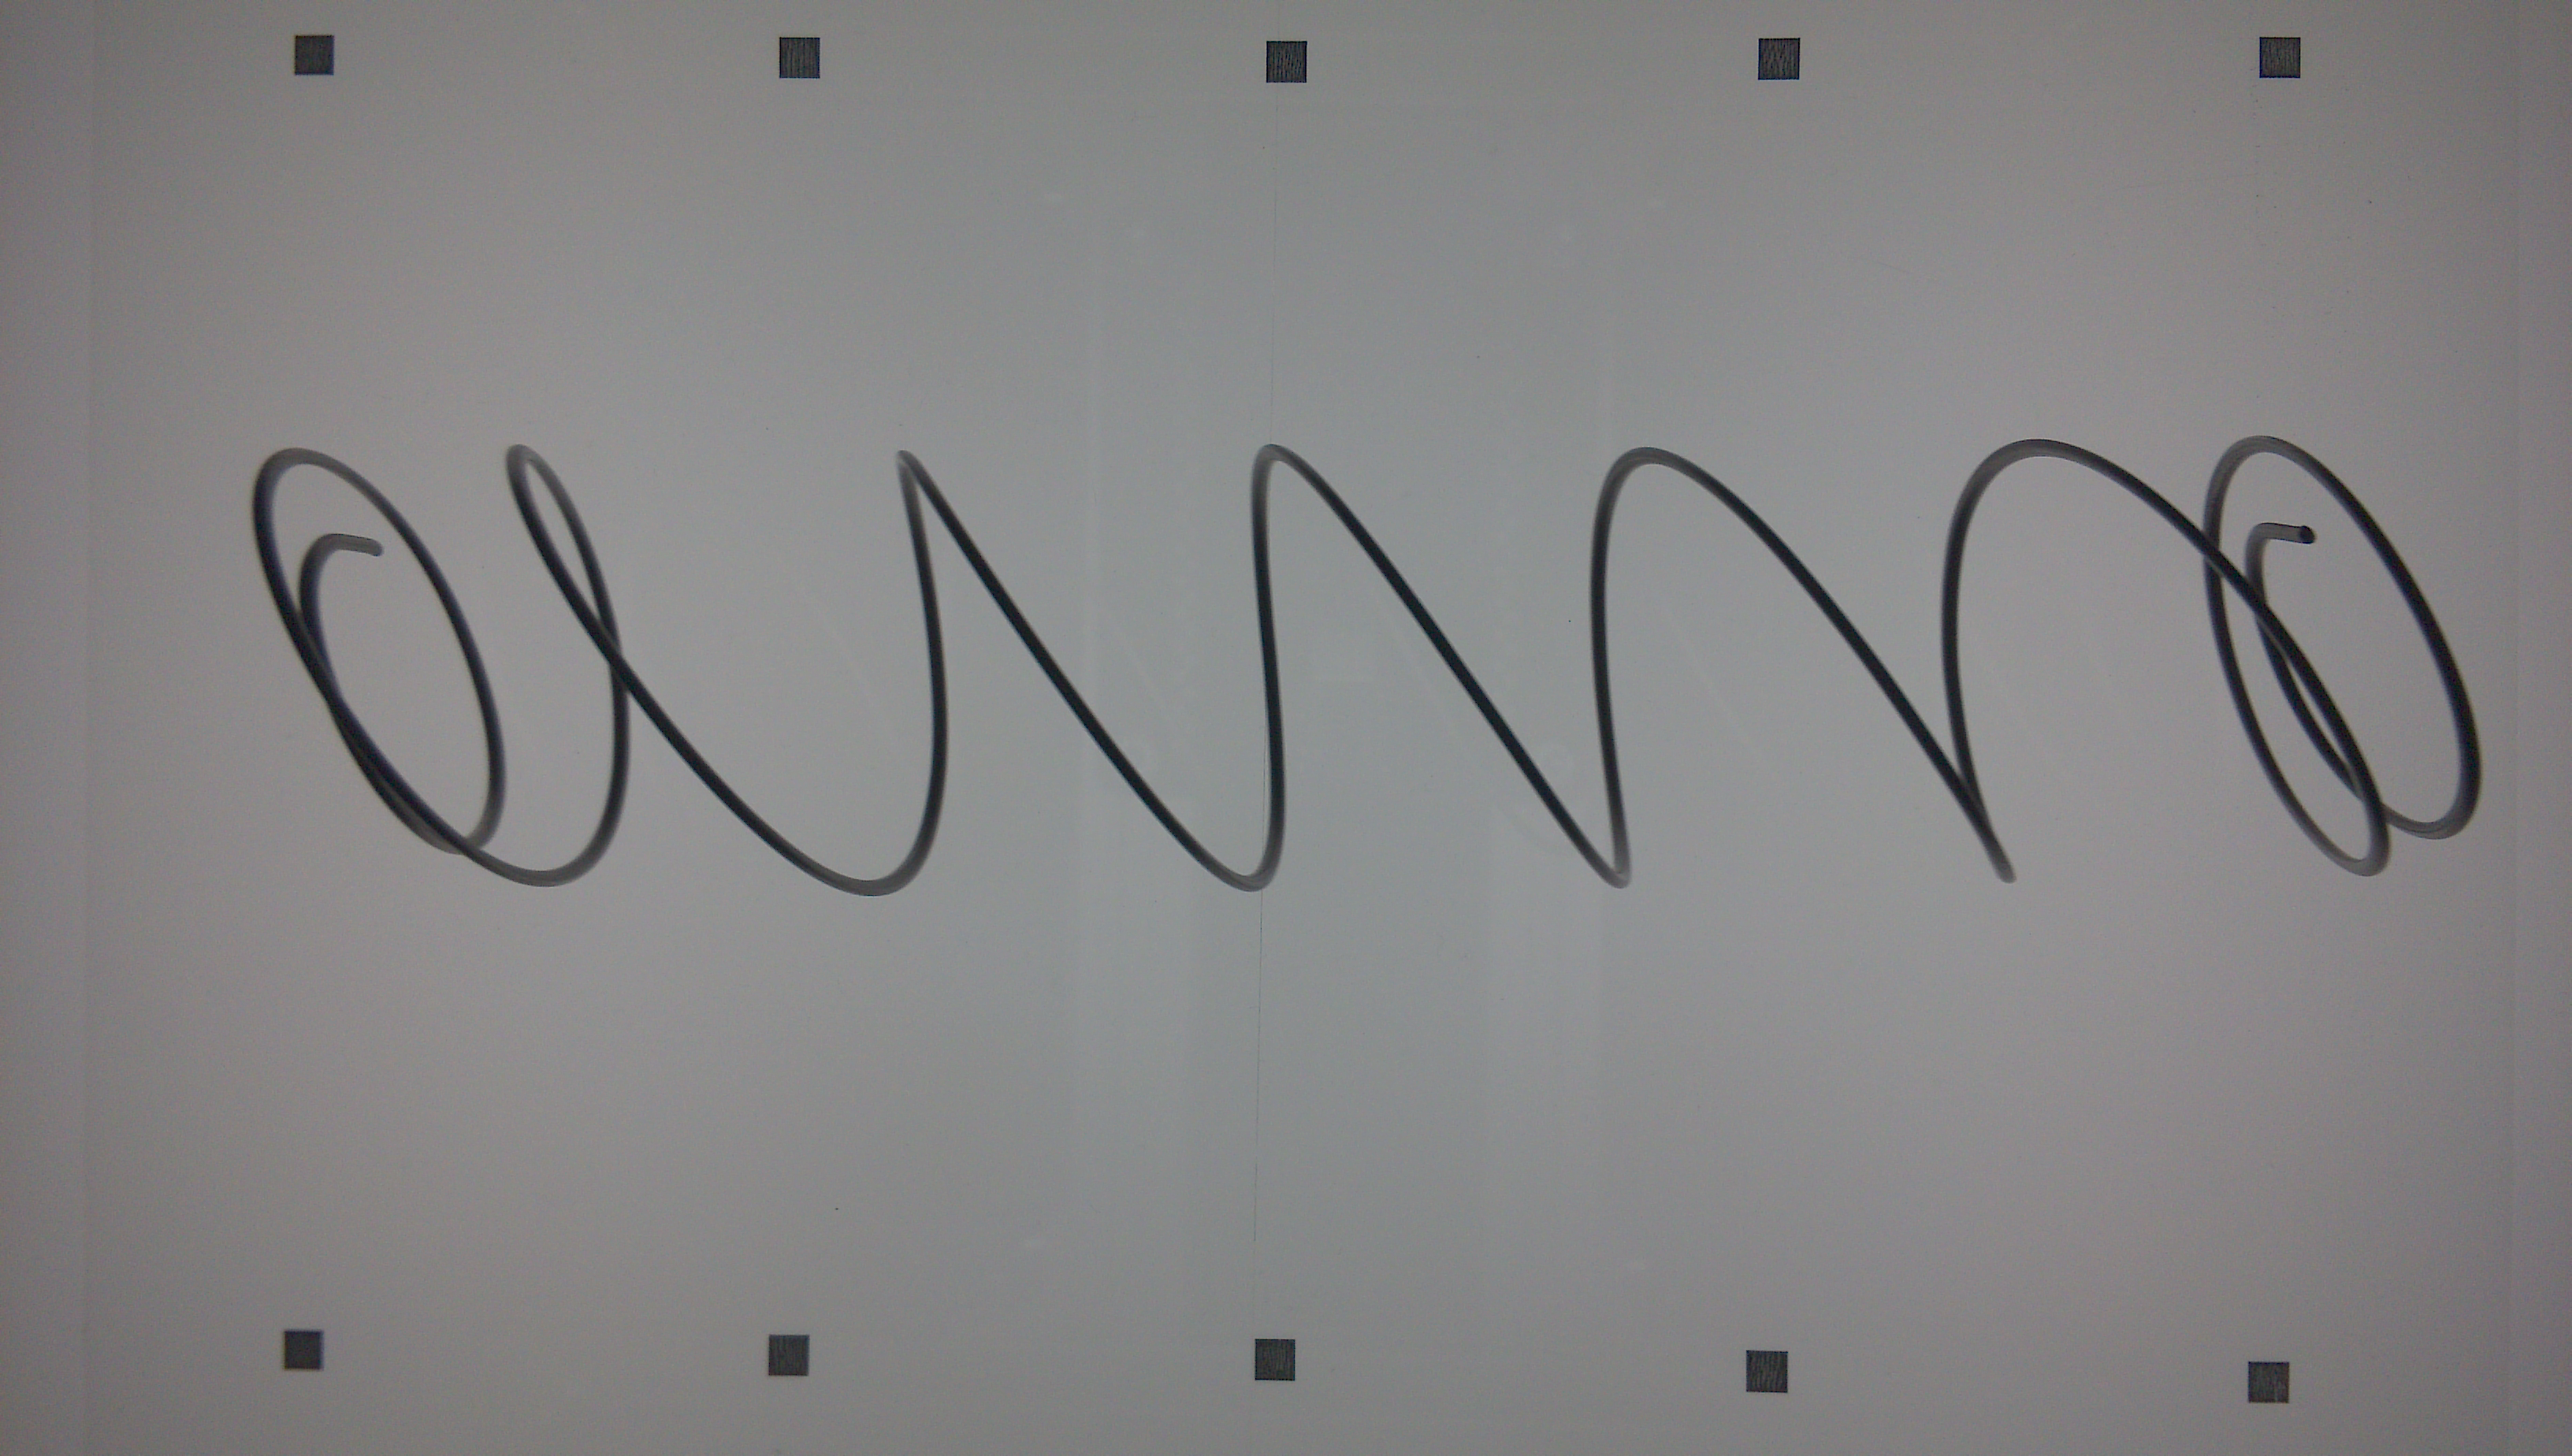
\includegraphics[width=0.9\textwidth]{3-development/software/images/rolling.png}
	\caption{Rolling shutter effect on a spring moving through the frame (left to right).\label{development:rolling}}
\end{figure}
Making measurements with this image makes it necessary to correct the length.
 

